\chapter{Deployment}
\label{cha:deployment}

\section{Github Organization} % (fold)
\label{sec:github}

This project and all its components belong to a github organization called \texttt{xmlet0}\footnote{\href{https://github.com/xmlet}{xmlet Github}}. The aim of that organization is to contain all the related projects to this dissertation. All the generated \ac{API}s are also created as if they belong to this organization. 

\section{Maven} % (fold)
\label{sec:maven}

In order to manage the developed projects a tool for project organization and deployment was used, named Maven. Maven has the goal of organizing a project in many different ways, such as creating a standard of project building and managing project dependencies. Maven was also used to generate documentation and deploying the projects to a central code repository, Maven Central Repository\footnote{\href{https://search.maven.org/}{Maven Central Repository}}. All the releases of projects belonging to the \texttt{xmlet} Github organization can be found under using the artifactId, \href{https://search.maven.org/#search%7Cga%7C1%7Ccom.github.xmlet}{com.github.xmlet}. 

\section{Sonarcloud} % (fold)
\label{sec:sonarcloud}

Code quality and its various implications such as security, low performance and bugs should always be an important issue to a programmer. With that in mind all the projects contained in the \texttt{xmlet} solution were evaluated in various metrics and the results made public for consultation. This way, either future users of those projects or developers trying to improve the projects can check the metrics as another way of validating the quality of the produced code. The tool to perform this evaluation was Sonarcloud\footnote{\href{https://sonarcloud.io/organizations/xmlet/projects}{Sonarcloud xmlet page}}, which provides free of charge evaluations and stores the results which are available for everyone.

\section{Testing metrics} % (fold)
\label{sec:testingmetrics}

Perform efficiency tests comparing the HtmlApi, j2html and Apache Velocity. The test should be based on a html page with multiple elements and attributes, probably the test should be performed with different number of html elements, like 10, 50, 100, 1000.

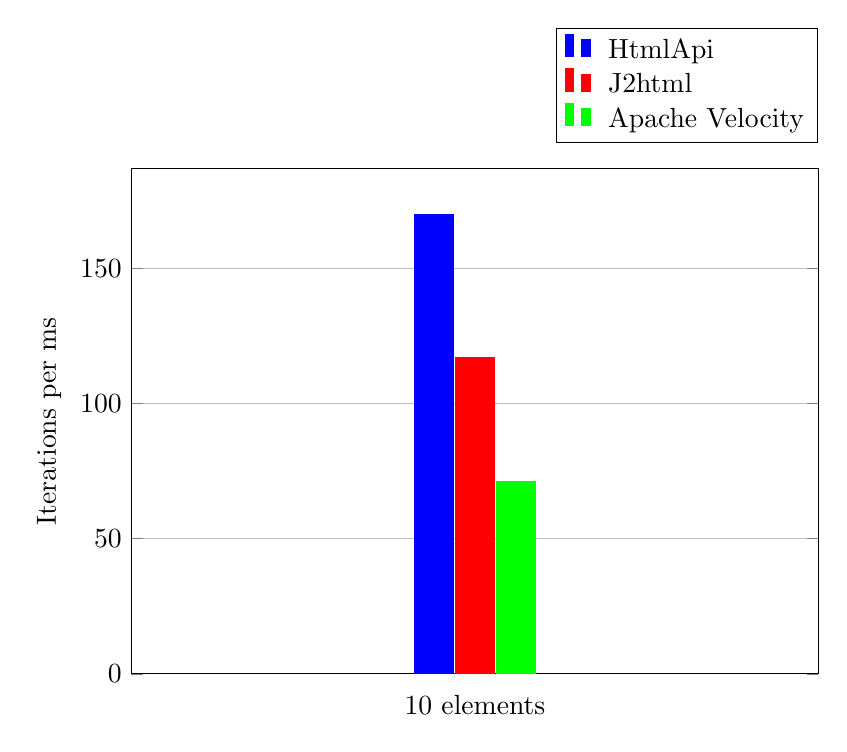
\begin{tikzpicture}
    \begin{axis}[
        width  = 0.85*\textwidth,
        height = 8cm,
        major x tick style = transparent,
        ybar=2*\pgflinewidth,
        bar width=14pt,
        ymajorgrids = true,
        ylabel = {Iterations per ms},
		symbolic x coords={10 elements},
        xtick = data,
        scaled y ticks = false,
        enlarge x limits=0.25,
        ymin=0,
        legend cell align=left,
        legend style={
                at={(1,1.05)},
                anchor=south east,
                column sep=1ex
        }
    ]
        \addplot[style={blue,fill=blue,mark=none}]
            coordinates {(10 elements, 170)};

        \addplot[style={red,fill=red,mark=none}]
             coordinates {(10 elements, 117)};

        \addplot[style={green,fill=green,mark=none}]
             coordinates {(10 elements, 71)};

        \legend{HtmlApi,J2html,Apache Velocity}
    \end{axis}
\end{tikzpicture}


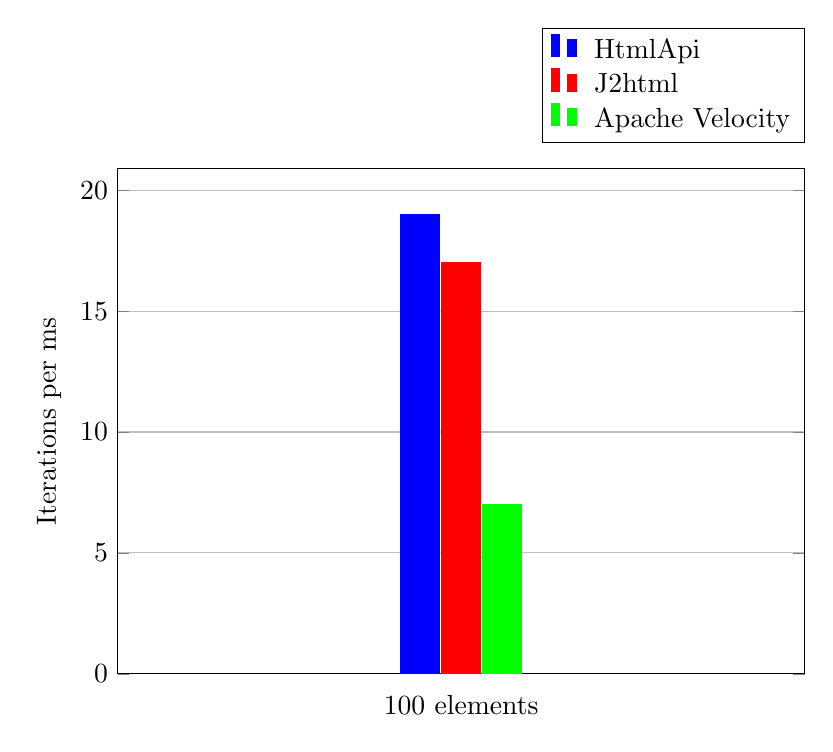
\begin{tikzpicture}
    \begin{axis}[
        width  = 0.85*\textwidth,
        height = 8cm,
        major x tick style = transparent,
        ybar=2*\pgflinewidth,
        bar width=14pt,
        ymajorgrids = true,
        ylabel = {Iterations per ms},
		symbolic x coords={100 elements},
        xtick = data,
        scaled y ticks = false,
        enlarge x limits=0.25,
        ymin=0,
        legend cell align=left,
        legend style={
                at={(1,1.05)},
                anchor=south east,
                column sep=1ex
        }
    ]
        \addplot[style={blue,fill=blue,mark=none}]
            coordinates {(100 elements, 19)};

        \addplot[style={red,fill=red,mark=none}]
             coordinates {(100 elements, 17)};

        \addplot[style={green,fill=green,mark=none}]
             coordinates {(100 elements, 7)};

        \legend{HtmlApi,J2html,Apache Velocity}
    \end{axis}
\end{tikzpicture}


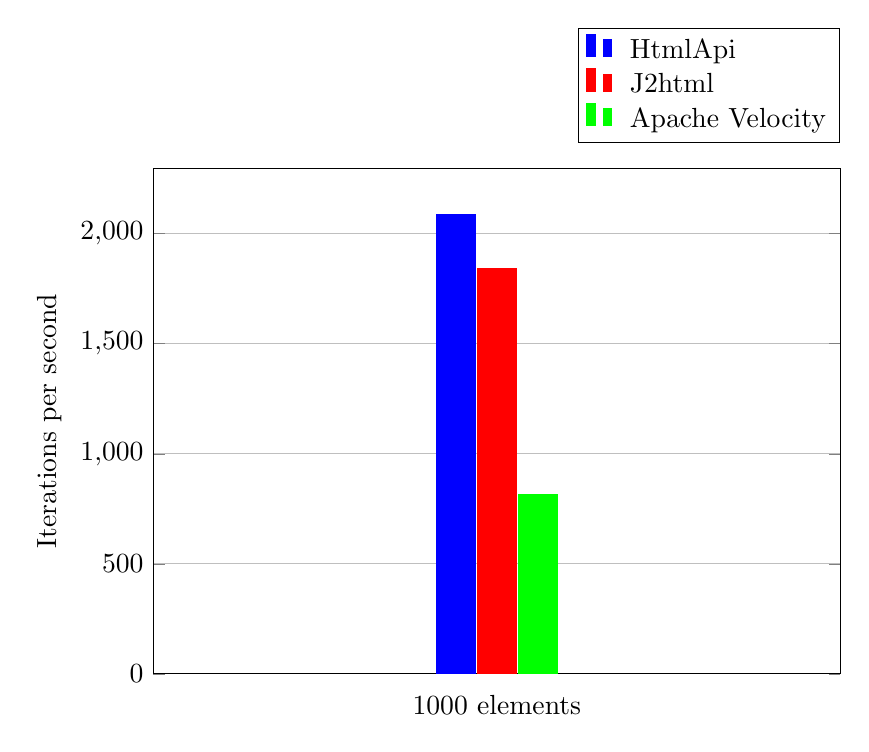
\begin{tikzpicture}
    \begin{axis}[
        width  = 0.85*\textwidth,
        height = 8cm,
        major x tick style = transparent,
        ybar=2*\pgflinewidth,
        bar width=14pt,
        ymajorgrids = true,
        ylabel = {Iterations per second},
		symbolic x coords={1000 elements},
        xtick = data,
        scaled y ticks = false,
        enlarge x limits=0.25,
        ymin=0,
        legend cell align=left,
        legend style={
                at={(1,1.05)},
                anchor=south east,
                column sep=1ex
        }
    ]
        \addplot[style={blue,fill=blue,mark=none}]
            coordinates {(1000 elements, 2088)};

        \addplot[style={red,fill=red,mark=none}]
             coordinates {(1000 elements, 1842)};

        \addplot[style={green,fill=green,mark=none}]
             coordinates {(1000 elements, 813)};

        \legend{HtmlApi,J2html,Apache Velocity}
    \end{axis}
\end{tikzpicture}


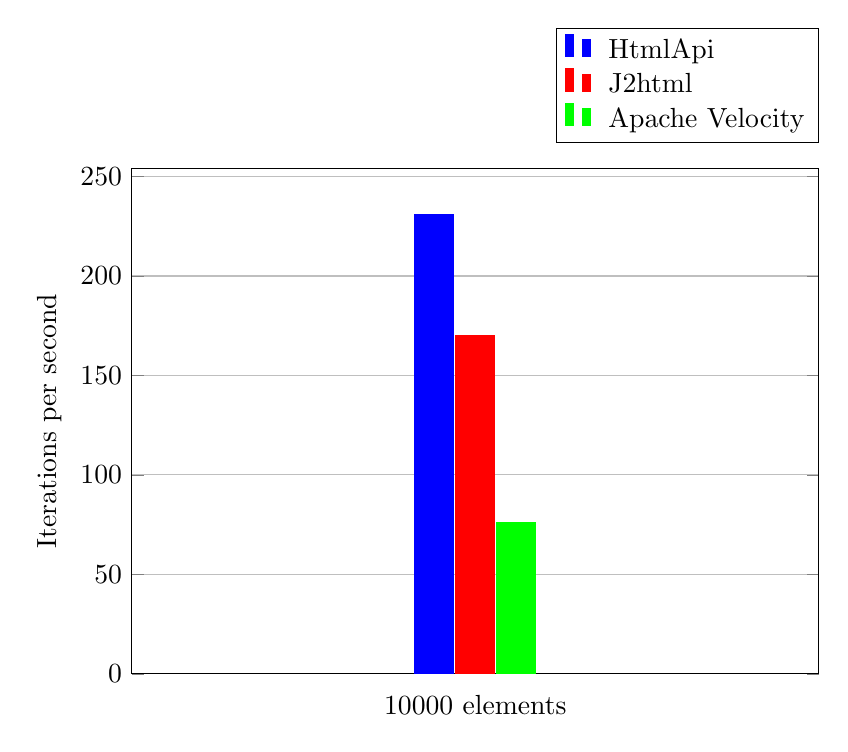
\begin{tikzpicture}
    \begin{axis}[
        width  = 0.85*\textwidth,
        height = 8cm,
        major x tick style = transparent,
        ybar=2*\pgflinewidth,
        bar width=14pt,
        ymajorgrids = true,
        ylabel = {Iterations per second},
		symbolic x coords={10000 elements},
        xtick = data,
        scaled y ticks = false,
        enlarge x limits=0.25,
        ymin=0,
        legend cell align=left,
        legend style={
                at={(1,1.05)},
                anchor=south east,
                column sep=1ex
        }
    ]
        \addplot[style={blue,fill=blue,mark=none}]
            coordinates {(10000 elements, 231)};

        \addplot[style={red,fill=red,mark=none}]
             coordinates {(10000 elements, 170)};

        \addplot[style={green,fill=green,mark=none}]
             coordinates {(10000 elements, 76)};

        \legend{HtmlApi,J2html,Apache Velocity}
    \end{axis}
\end{tikzpicture}

%% Benchmark                           (elementCount)   Mode  Cnt       Score      Error  Units \\
%% htmlApiBenchmarkTableNoIndentation              10  thrpt    8  170328$693 ± 1614$096  ops/s \\
%% htmlApiBenchmarkTableNoIndentation             100  thrpt    8   19741$036 ±   51$216  ops/s \\
%% htmlApiBenchmarkTableNoIndentation            1000  thrpt    8    2088$301 ±   11$389  ops/s \\
%% htmlApiBenchmarkTableNoIndentation           10000  thrpt    8     231$082 ±    2$331  ops/s \\
%%  
%% J2html / Apache Velocity \\
%%  
%% j2htmlBenchmark                                 10  thrpt    8  117115$030 ± 1271$023  ops/s \\
%% j2htmlBenchmark                                100  thrpt    8   17911$202 ±   50$985  ops/s \\
%% j2htmlBenchmark                               1000  thrpt    8    1842$156 ±    4$667  ops/s \\
%% j2htmlBenchmark                              10000  thrpt    8     170$310 ±    1$490  ops/s \\
%% velocityBenchmark                               10  thrpt    8   71651$471 ±  477$994  ops/s \\
%% velocityBenchmark                              100  thrpt    8    7886$456 ±  204$865  ops/s \\
%% velocityBenchmark                             1000  thrpt    8     813$229 ±    3$891  ops/s \\
%% velocityBenchmark                            10000  thrpt    8      76$934 ±    0$795  ops/s \\
%%  
%% In Depth w/ char [] \\
%%  
%% htmlApiBenchmarkDivs                            10  thrpt    8   96242$098 ±  358$183  ops/s \\
%% htmlApiBenchmarkDivs                           100  thrpt    8    4871$983 ±   15$870  ops/s \\
%% htmlApiBenchmarkDivsNoIndentation               10  thrpt    8  153090$042 ± 5601$598  ops/s \\
%% htmlApiBenchmarkDivsNoIndentation              100  thrpt    8   20894$867 ±   54$526  ops/s \\
%% 
%% With indentation
%% 
%% htmlApiBenchmarkTable                           10  thrpt    8  131608$951 ±  2366$956  ops/s \\
%% htmlApiBenchmarkTable                          100  thrpt    8   15414$713 ±   110$575  ops/s \\
%% htmlApiBenchmarkTable                         1000  thrpt    8    1562$108 ±    53$736  ops/s \\
%% htmlApiBenchmarkTable                        10000  thrpt    8     174$760 ±     1$149  ops/s \\